\section{Тестирование программы}
\setcounter{figure}{0}

\subsection{Тесты консоли администратора}

Запустим консоль и введём неверный пароль.

Ожидается, что программа завершится с сообщением Incorrect password!
(рис. \ref{bad_pass})

\begin{figure}[H]
	\centering
	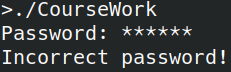
\includegraphics[width=0.7\linewidth]{photo/tests/admin/bad_pass}
	\caption{Тест -- неверный пароль}
	\label{bad_pass}
\end{figure}

Запустим консоль и введём пароль. Выберем базу грузовиков и распечатаем её.

Ожидается, что программа выведет текущее состояние базы данных.
Исходный файл с базой на рис. \ref{truck_db_state_init}.
Результат выполнения на рис. \ref{truck_db_print}.

\begin{figure}[H]
	\centering
	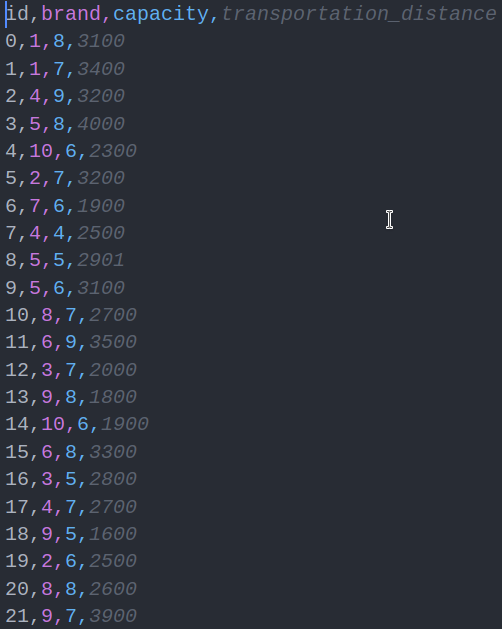
\includegraphics[width=0.5\linewidth]{photo/tests/admin/truck_db_state_init}
	\caption{Тест -- Файл базы данных грузовиков}
	\label{truck_db_state_init}
\end{figure}

\begin{figure}[H]
	\centering
	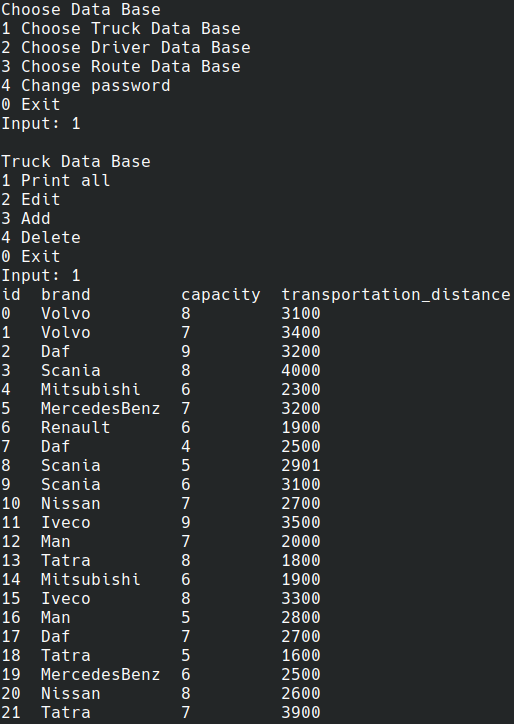
\includegraphics[width=0.7\linewidth]{photo/tests/admin/truck_db_print}
	\caption{Тест -- Вывод базы данных грузовиков}
	\label{truck_db_print}
\end{figure}

Запустим консоль и введём пароль. Выберем базу грузовиков добавим новую запись.

Ожидается, что программа добавит новый элемент в файл базы данных.
Исходный файл с базой до изменений на рис. \ref{truck_db_state_init2}.
Результат выполнения на рис. \ref{truck_db_add}.
Исходный файл с базой после изменений на рис. \ref{truck_db_state_add}.

\begin{figure}[H]
	\centering
	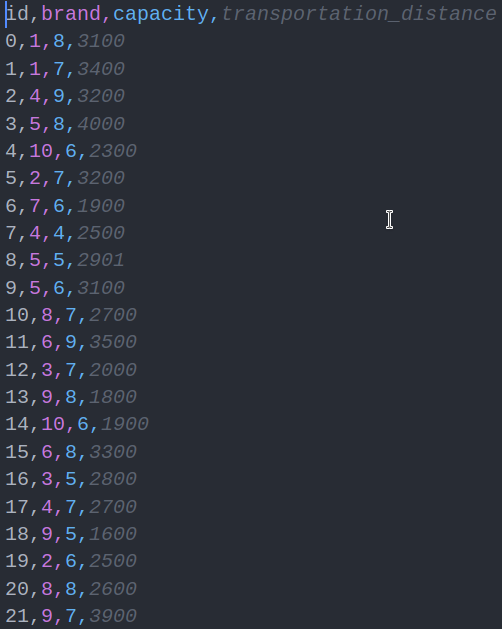
\includegraphics[width=0.4\linewidth]{photo/tests/admin/truck_db_state_init}
	\caption{Тест -- Файл базы данных грузовиков до изменений}
	\label{truck_db_state_init2}
\end{figure}

\begin{figure}[H]
	\centering
	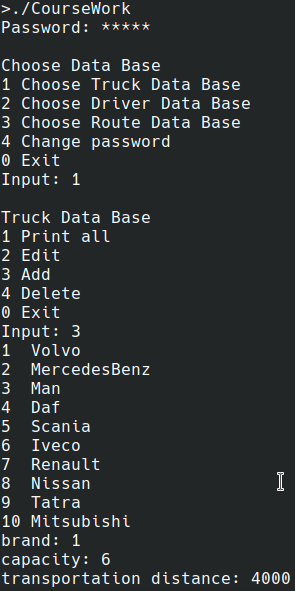
\includegraphics[width=0.4\linewidth]{photo/tests/admin/truck_db_add}
	\caption{Тест -- Добавление записи в базу грузовиков}
	\label{truck_db_add}
\end{figure}

\begin{figure}[H]
	\centering
	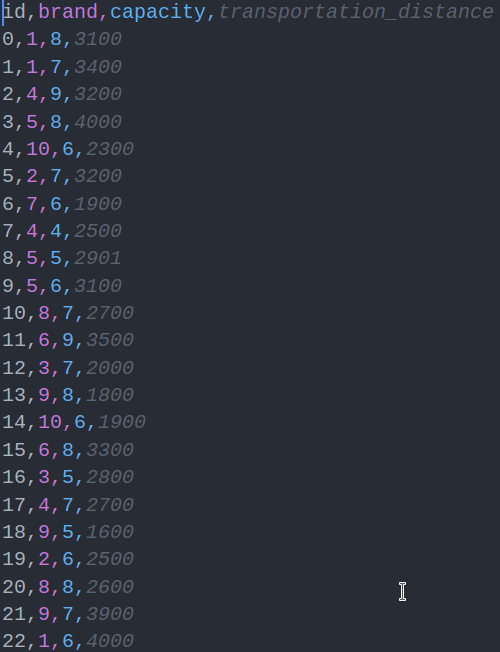
\includegraphics[width=0.5\linewidth]{photo/tests/admin/truck_db_state_add}
	\caption{Тест -- Файл базы данных грузовиков после изменений}
	\label{truck_db_state_add}
\end{figure}

Запустим консоль и введём пароль. 
Выберем базу грузовиков и отредактируем новую запись,
изменив модель грузовика на Iveco, 
грузоподъёмность на 8 и 
максимальную дистанцию поставки на 4500.

Ожидается, что программа изменит элемент в файле базы данных.
Исходный файл с базой до изменений на рис. \ref{truck_db_state_add2}.
Результат выполнения на рис. \ref{truck_db_edit}.
Исходный файл с базой после изменений на рис. \ref{truck_db_state_edit}.

\begin{figure}[H]
	\centering
	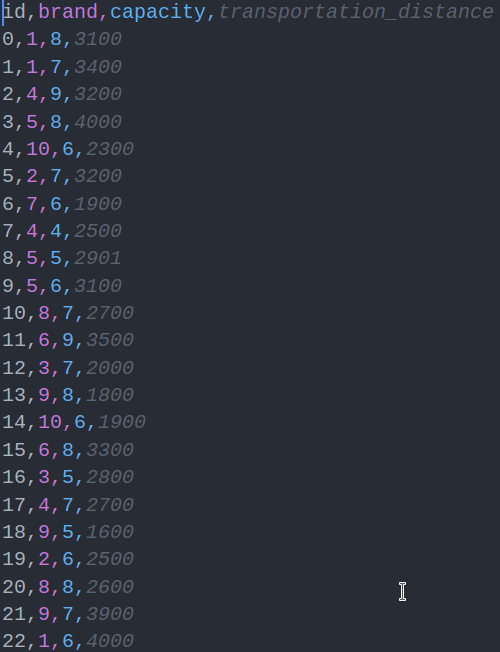
\includegraphics[width=0.7\linewidth]{photo/tests/admin/truck_db_state_add}
	\caption{Тест -- Файл базы данных грузовиков до изменений}
	\label{truck_db_state_add2}
\end{figure}

\begin{figure}[H]
	\centering
	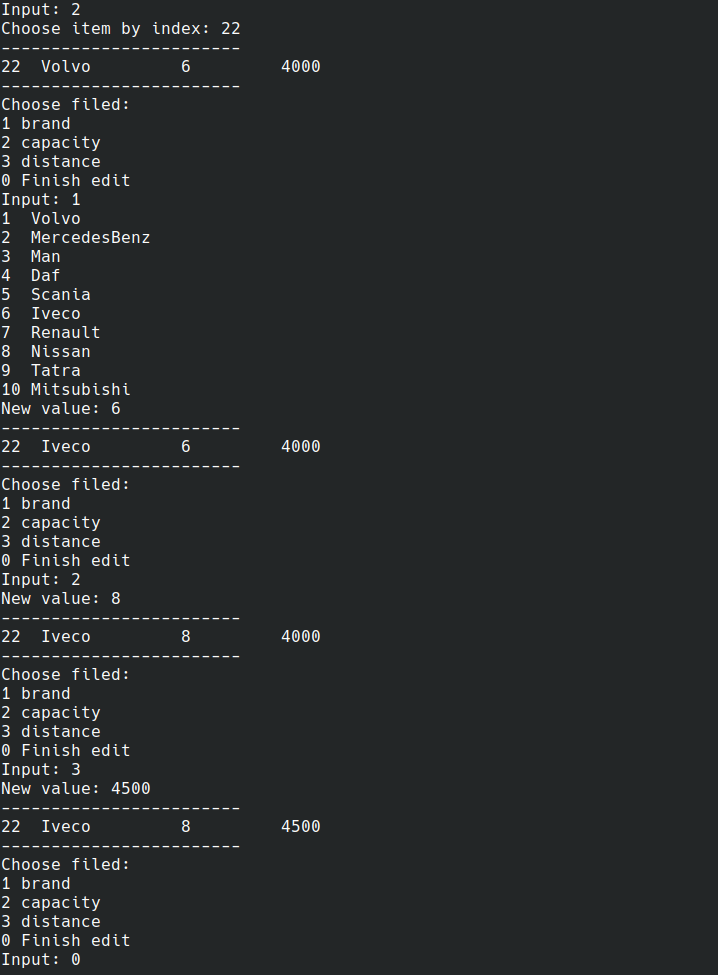
\includegraphics[width=0.8\linewidth]{photo/tests/admin/truck_db_edit}
	\caption{Тест -- Редактирование записи из базы грузовиков}
	\label{truck_db_edit}
\end{figure}

\begin{figure}[H]
	\centering
	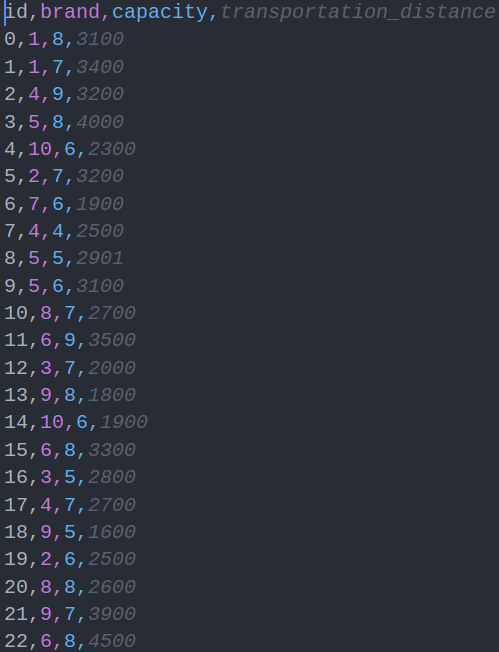
\includegraphics[width=0.7\linewidth]{photo/tests/admin/truck_db_state_edit}
	\caption{Тест -- Файл базы данных грузовиков после изменений}
	\label{truck_db_state_edit}
\end{figure}

Запустим консоль и введём пароль. 
Выберем базу грузовиков и удалим запись

Ожидается, что программа удалит элемент из файла базы данных.
Исходный файл с базой до изменений на рис. \ref{truck_db_state_edit2}.
Результат выполнения на рис. \ref{truck_db_delete}.
Исходный файл с базой после изменений на рис. \ref{truck_db_state_init3}.

\begin{figure}[H]
	\centering
	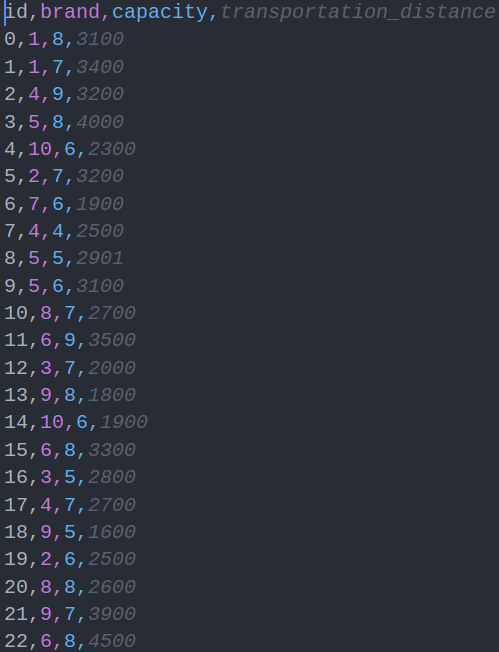
\includegraphics[width=0.7\linewidth]{photo/tests/admin/truck_db_state_edit}
	\caption{Тест -- Файл базы данных грузовиков до изменений}
	\label{truck_db_state_edit2}
\end{figure}

\begin{figure}[H]
	\centering
	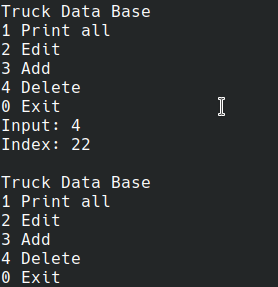
\includegraphics[width=0.8\linewidth]{photo/tests/admin/truck_db_delete}
	\caption{Тест -- Удаление записи из базы грузовиков}
	\label{truck_db_delete}
\end{figure}

\begin{figure}[H]
	\centering
	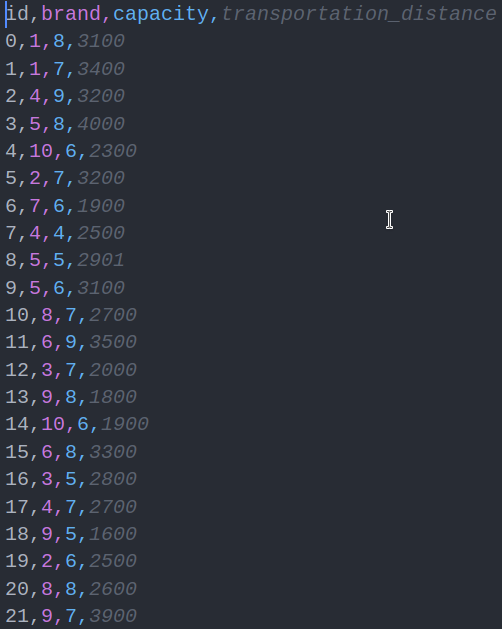
\includegraphics[width=0.7\linewidth]{photo/tests/admin/truck_db_state_init}
	\caption{Тест -- Файл базы данных грузовиков после изменений}
	\label{truck_db_state_init3}
\end{figure}

%%%%%%%%%%%%%%%%%%%%%%%%%%%%%%%%%%%%%%%%%%%%%%%%%%%%%%%%%%%%%%%%%%%%%%%%%%%%%%%%%%%%%%%%
% DRIVER	DRIVER	DRIVER	DRIVER	DRIVER	DRIVER	DRIVER	DRIVER	DRIVER	DRIVER	
%%%%%%%%%%%%%%%%%%%%%%%%%%%%%%%%%%%%%%%%%%%%%%%%%%%%%%%%%%%%%%%%%%%%%%%%%%%%%%%%%%%%%%%%

Запустим консоль и введём пароль. 
Выберем базу водителей и распечатаем её.

Ожидается, что программа выведет текущее состояние базы данных.
Исходный файл с базой на рис. \ref{driver_db_state_init}.
Результат выполнения на рис. \ref{driver_db_print}.

\begin{figure}[H]
	\centering
	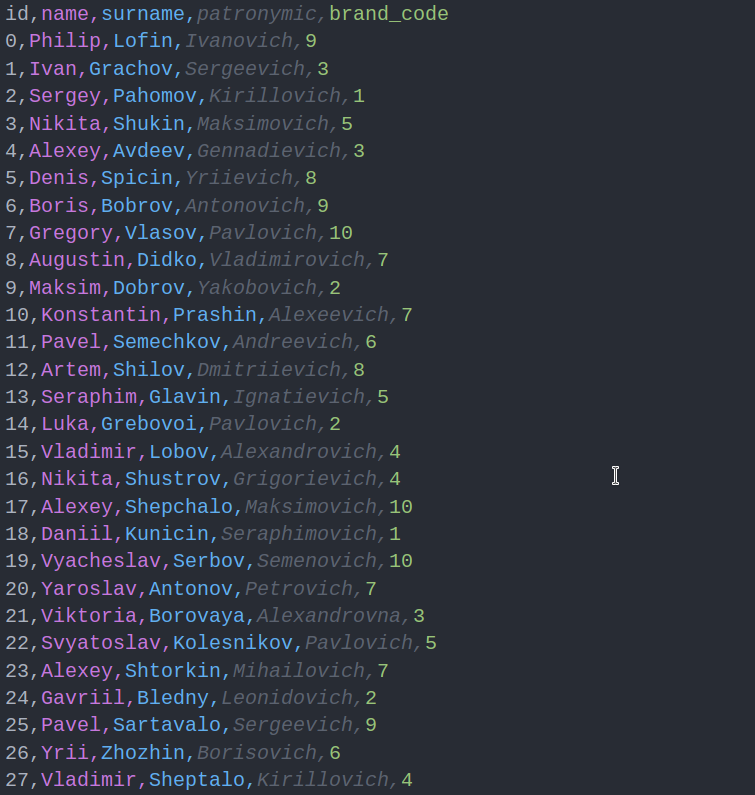
\includegraphics[width=0.7\linewidth]{photo/tests/admin/driver_db_state_init}
	\caption{Тест -- Файл базы данных водителей}
	\label{driver_db_state_init}
\end{figure}

\begin{figure}[H]
	\centering
	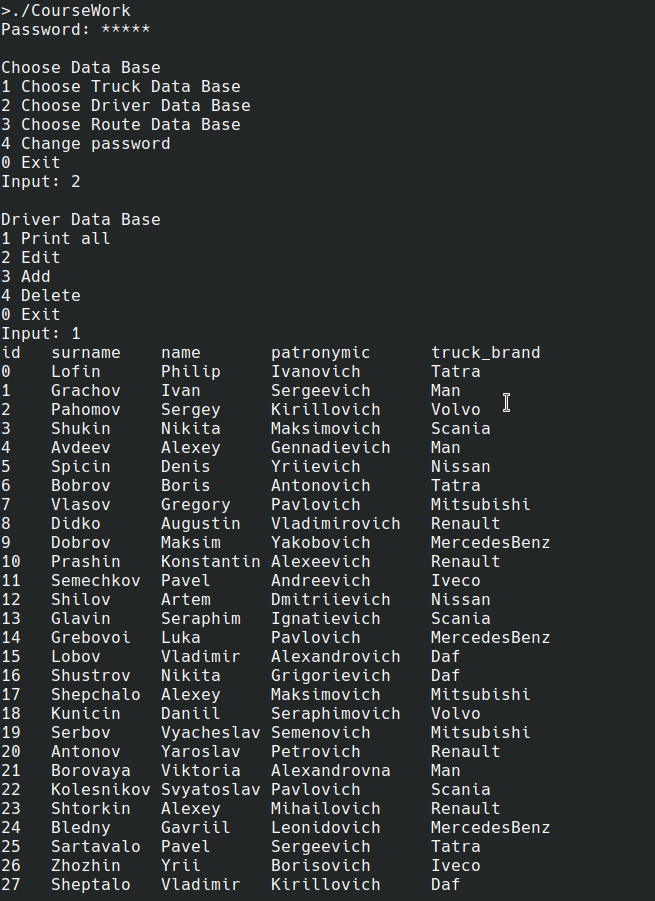
\includegraphics[width=0.7\linewidth]{photo/tests/admin/driver_db_print}
	\caption{Тест -- Вывод базы данных водителей}
	\label{driver_db_print}
\end{figure}

Запустим консоль и введём пароль. 
Выберем базу водителей добавим новую запись.

Ожидается, что программа добавит новый элемент в файл базы данных.
Исходный файл с базой до изменений на рис. \ref{driver_db_state_init2}.
Результат выполнения на рис. \ref{driver_db_add}.
Исходный файл с базой после изменений на рис. \ref{driver_db_state_add}.

\begin{figure}[H]
	\centering
	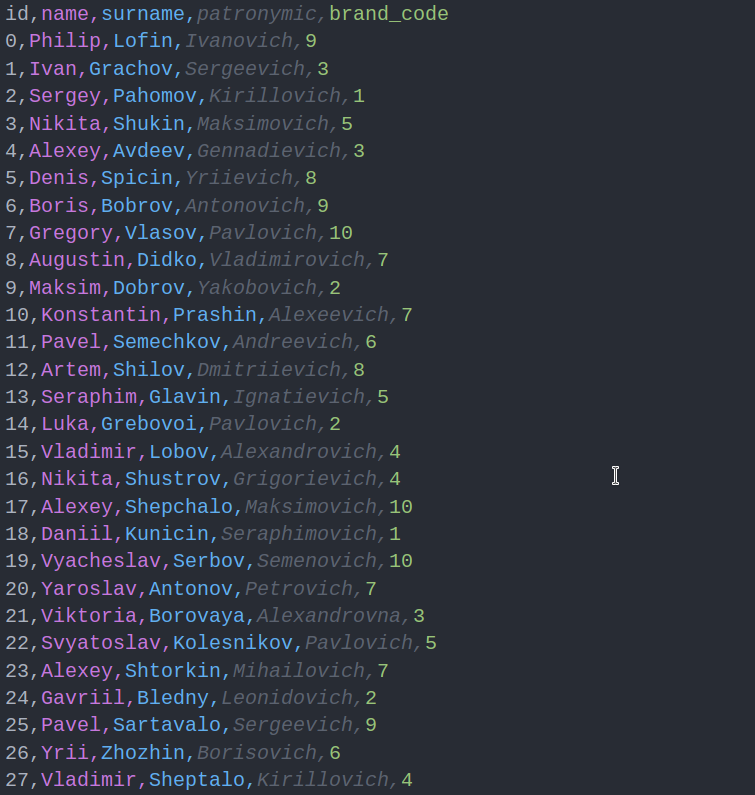
\includegraphics[width=0.7\linewidth]{photo/tests/admin/driver_db_state_init}
	\caption{Тест -- Файл базы данных водителей до изменений}
	\label{driver_db_state_init2}
\end{figure}

\begin{figure}[H]
	\centering
	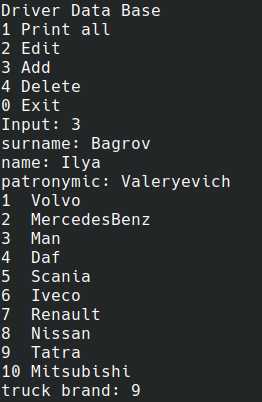
\includegraphics[width=0.4\linewidth]{photo/tests/admin/driver_db_add}
	\caption{Тест -- Добавление записи в базу водителей}
	\label{driver_db_add}
\end{figure}

\begin{figure}[H]
	\centering
	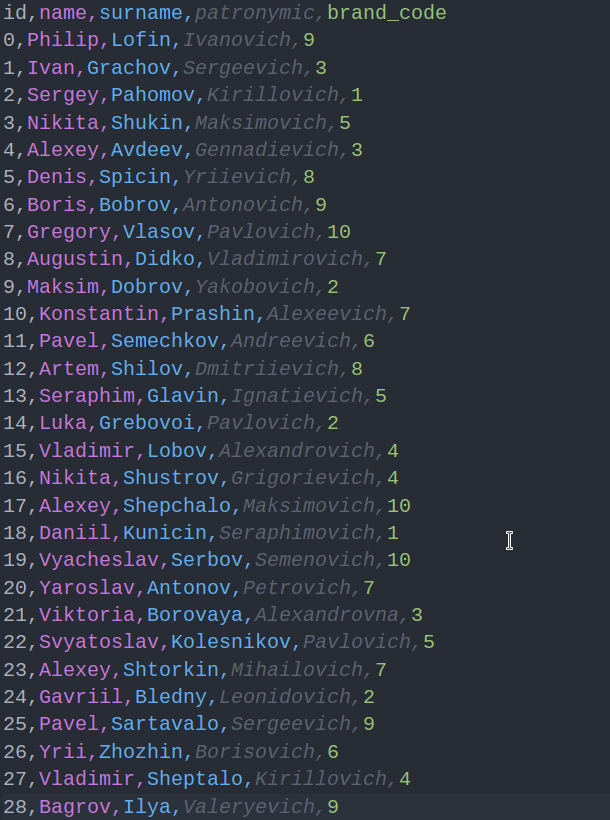
\includegraphics[width=0.5\linewidth]{photo/tests/admin/driver_db_state_add}
	\caption{Тест -- Файл базы данных водителей после изменений}
	\label{driver_db_state_add}
\end{figure}

Запустим консоль и введём пароль. 
Выберем базу водителей и отредактируем новую запись,
изменив 
имя на Sergey,
фамилию на Borovin,
отчество на Pavlovich,
марку на Volvo.

Ожидается, что программа изменит элемент в файле базы данных.
Исходный файл с базой до изменений на рис. \ref{driver_db_state_add2}.
Результат выполнения на рис. \ref{driver_db_edit_1}, \ref{driver_db_edit_2}.
Исходный файл с базой после изменений на рис. \ref{driver_db_state_edit}.

\begin{figure}[H]
	\centering
	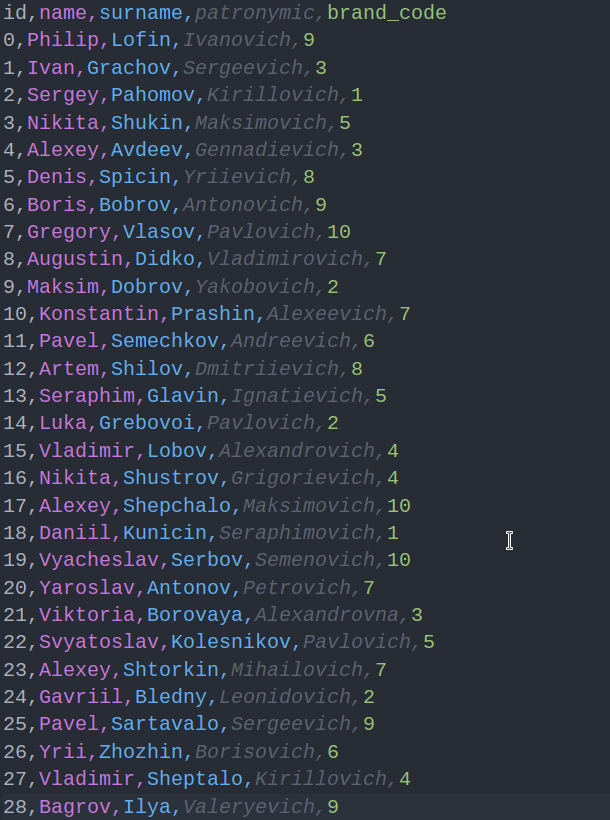
\includegraphics[width=0.7\linewidth]{photo/tests/admin/driver_db_state_add}
	\caption{Тест -- Файл базы данных водителей до изменений}
	\label{driver_db_state_add2}
\end{figure}

\begin{figure}[H]
	\centering
	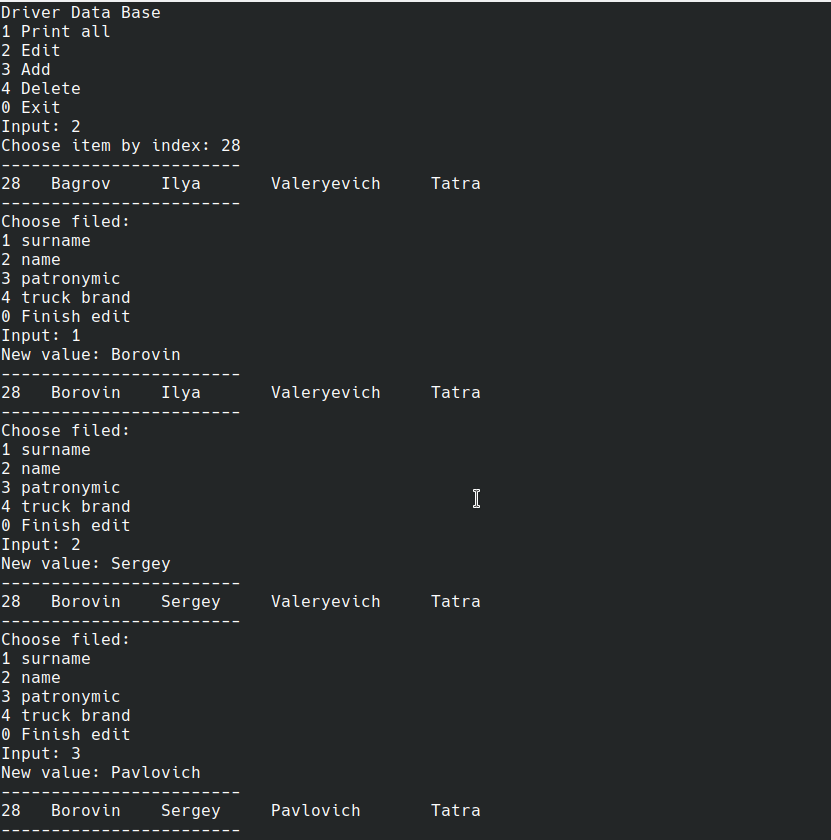
\includegraphics[width=0.8\linewidth]{photo/tests/admin/driver_db_edit_1}
	\caption{Тест -- Редактирование записи из базы водителей (1)}
	\label{driver_db_edit_1}
\end{figure}

\begin{figure}[H]
	\centering
	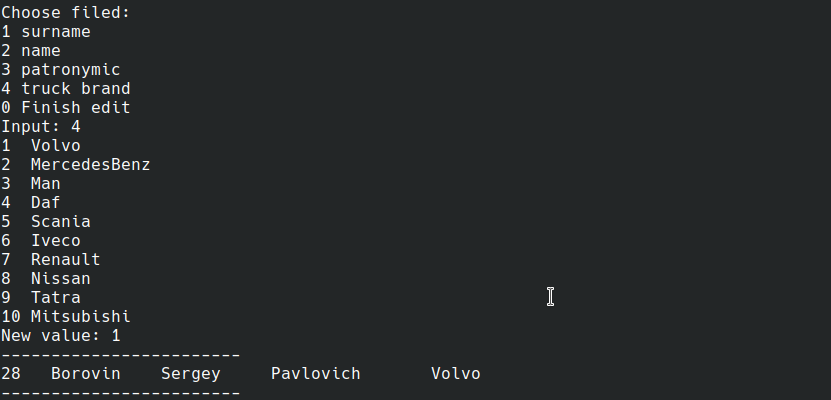
\includegraphics[width=0.8\linewidth]{photo/tests/admin/driver_db_edit_2}
	\caption{Тест -- Редактирование записи из базы водителей (2)}
	\label{driver_db_edit_2}
\end{figure}

\begin{figure}[H]
	\centering
	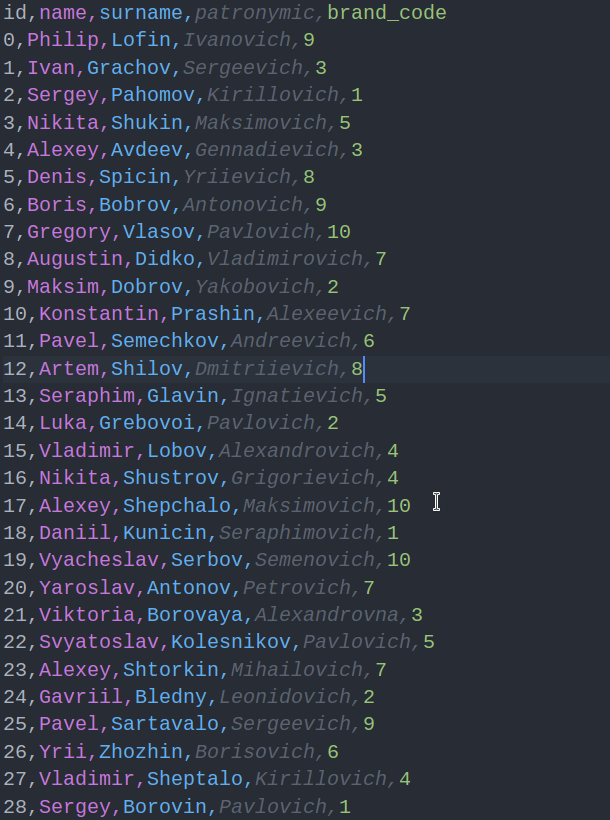
\includegraphics[width=0.7\linewidth]{photo/tests/admin/driver_db_state_edit}
	\caption{Тест -- Файл базы данных водителей после изменений}
	\label{driver_db_state_edit}
\end{figure}

Запустим консоль и введём пароль. 
Выберем базу водителей и удалим запись

Ожидается, что программа удалит элемент из файла базы данных.
Исходный файл с базой до изменений на рис. \ref{driver_db_state_edit2}.
Результат выполнения на рис. \ref{driver_db_delete}.
Исходный файл с базой после изменений на рис. \ref{driver_db_state_init3}.

\begin{figure}[H]
	\centering
	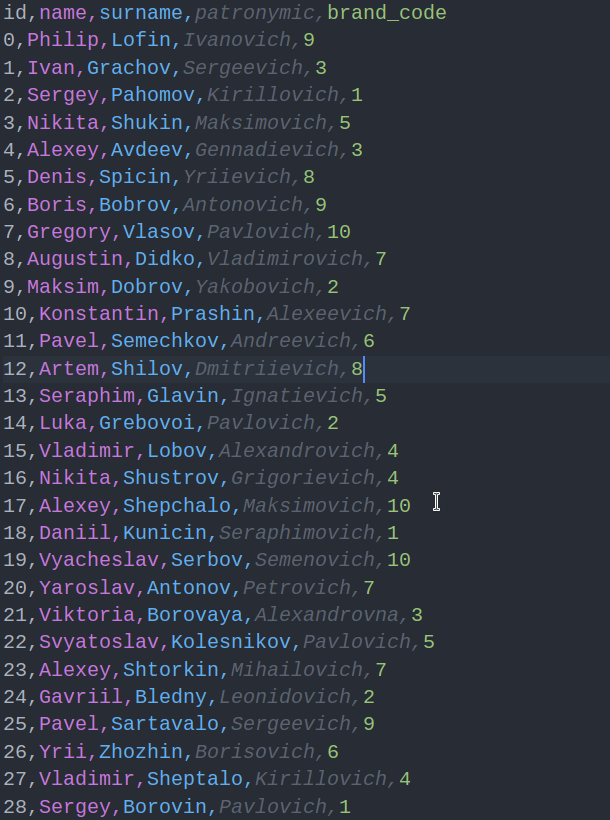
\includegraphics[width=0.7\linewidth]{photo/tests/admin/driver_db_state_edit}
	\caption{Тест -- Файл базы данных водителей до изменений}
	\label{driver_db_state_edit2}
\end{figure}

\begin{figure}[H]
	\centering
	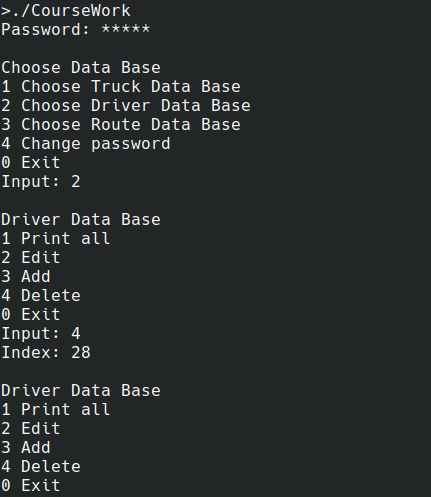
\includegraphics[width=0.8\linewidth]{photo/tests/admin/driver_db_delete}
	\caption{Тест -- Удаление записи из базы водителей}
	\label{driver_db_delete}
\end{figure}

\begin{figure}[H]
	\centering
	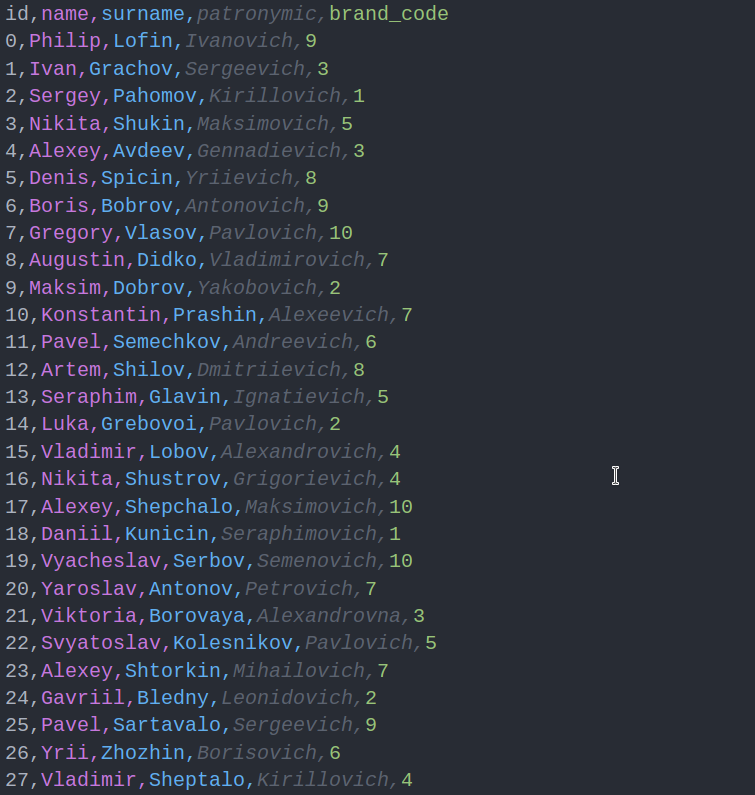
\includegraphics[width=0.7\linewidth]{photo/tests/admin/driver_db_state_init}
	\caption{Тест -- Файл базы данных водителей после изменений}
	\label{driver_db_state_init3}
\end{figure}

%%%%%%%%%%%%%%%%%%%%%%%%%%%%%%%%%%%%%%%%%%%%%%%%%%%%%%%%%%%%%%%%%%%%%%%%%%%%%%%%%%%%%%%%
% ROUTE	ROUTE	ROUTE	ROUTE	ROUTE	ROUTE	ROUTE	ROUTE	ROUTE	ROUTE	ROUTE
%%%%%%%%%%%%%%%%%%%%%%%%%%%%%%%%%%%%%%%%%%%%%%%%%%%%%%%%%%%%%%%%%%%%%%%%%%%%%%%%%%%%%%%%

Запустим консоль и введём пароль. 
Выберем базу маршрутов и распечатаем её.

Ожидается, что программа выведет текущее состояние базы данных.
Исходный файл с базой на рис. \ref{route_db_state_init}.
Результат выполнения на рис. \ref{route_db_print}.

\begin{figure}[H]
	\centering
	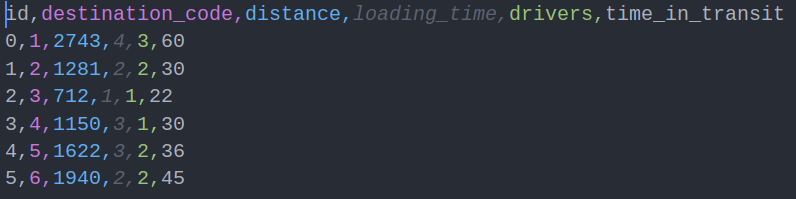
\includegraphics[width=0.7\linewidth]{photo/tests/admin/route_db_state_init}
	\caption{Тест -- Файл базы данных маршрутов}
	\label{route_db_state_init}
\end{figure}

\begin{figure}[H]
	\centering
	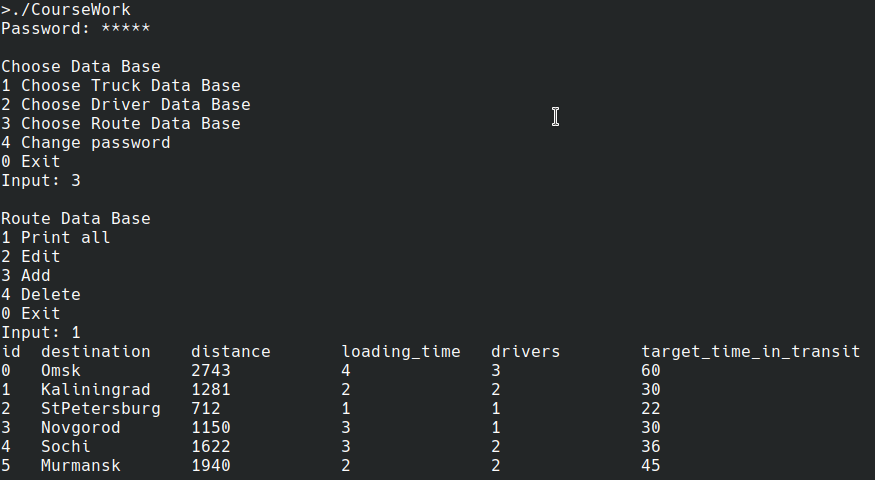
\includegraphics[width=0.7\linewidth]{photo/tests/admin/route_db_print}
	\caption{Тест -- Вывод базы данных маршрутов}
	\label{route_db_print}
\end{figure}

Запустим консоль и введём пароль. 
Выберем базу маршрутов добавим новую запись.

Ожидается, что программа добавит новый элемент в файл базы данных.
Исходный файл с базой до изменений на рис. \ref{route_db_state_init2}.
Результат выполнения на рис. \ref{route_db_add}.
Исходный файл с базой после изменений на рис. \ref{route_db_state_add}.

\begin{figure}[H]
	\centering
	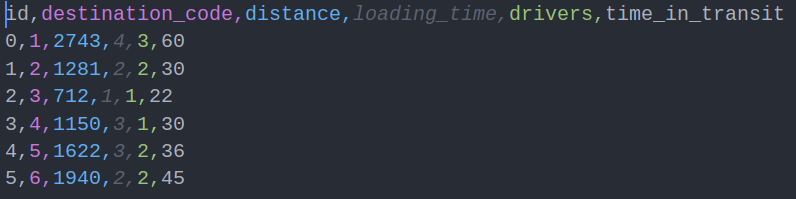
\includegraphics[width=0.7\linewidth]{photo/tests/admin/route_db_state_init}
	\caption{Тест -- Файл базы данных маршрутов до изменений}
	\label{route_db_state_init2}
\end{figure}

\begin{figure}[H]
	\centering
	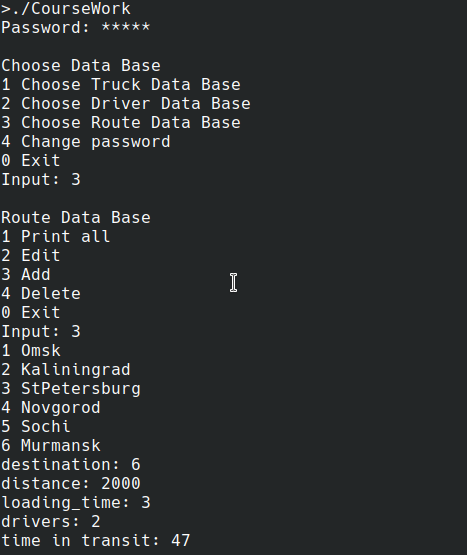
\includegraphics[width=0.4\linewidth]{photo/tests/admin/route_db_add}
	\caption{Тест -- Добавление записи в базу маршрутов}
	\label{route_db_add}
\end{figure}

\begin{figure}[H]
	\centering
	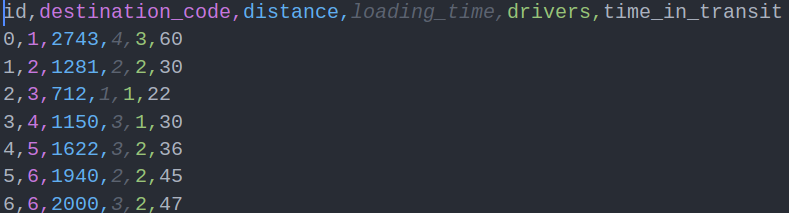
\includegraphics[width=0.5\linewidth]{photo/tests/admin/route_db_state_add}
	\caption{Тест -- Файл базы данных маршрутов после изменений}
	\label{route_db_state_add}
\end{figure}

Запустим консоль и введём пароль. 
Выберем базу маршрутов и отредактируем новую запись,
изменив 
коенчную точку на Sochi,
дистанцию на 1700,
время погрузки на 3,
количество водителей на 3 и 
время в пути в часах на 38.

Ожидается, что программа изменит элемент в файле базы данных.
Исходный файл с базой до изменений на рис. \ref{route_db_state_add2}.
Результат выполнения на рис. 
\ref{route_db_edit_1}, 
\ref{route_db_edit_2}, 
\ref{route_db_edit_3}.
Исходный файл с базой после изменений на рис. \ref{route_db_state_edit}.

\begin{figure}[H]
	\centering
	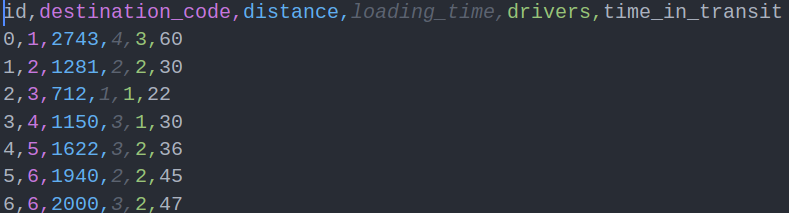
\includegraphics[width=0.7\linewidth]{photo/tests/admin/route_db_state_add}
	\caption{Тест -- Файл базы данных маршрутов до изменений}
	\label{route_db_state_add2}
\end{figure}

\begin{figure}[H]
	\centering
	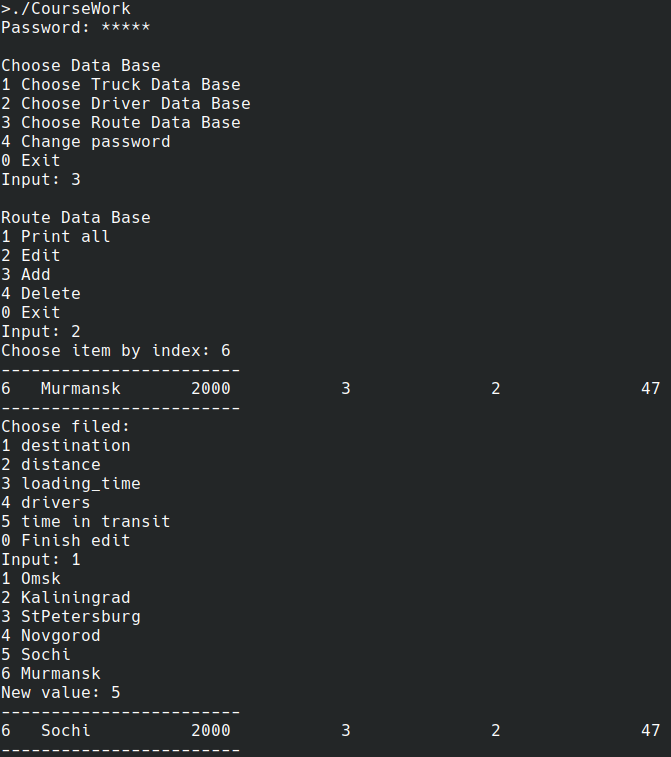
\includegraphics[width=0.8\linewidth]{photo/tests/admin/route_db_edit_1}
	\caption{Тест -- Редактирование записи из базы маршрутов (1)}
	\label{route_db_edit_1}
\end{figure}

\begin{figure}[H]
	\centering
	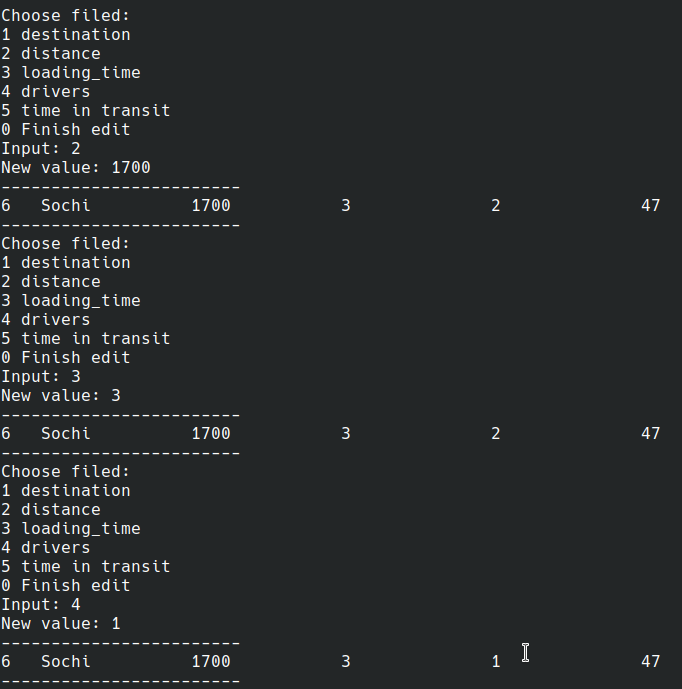
\includegraphics[width=0.8\linewidth]{photo/tests/admin/route_db_edit_2}
	\caption{Тест -- Редактирование записи из базы маршрутов (2)}
	\label{route_db_edit_2}
\end{figure}

\begin{figure}[H]
	\centering
	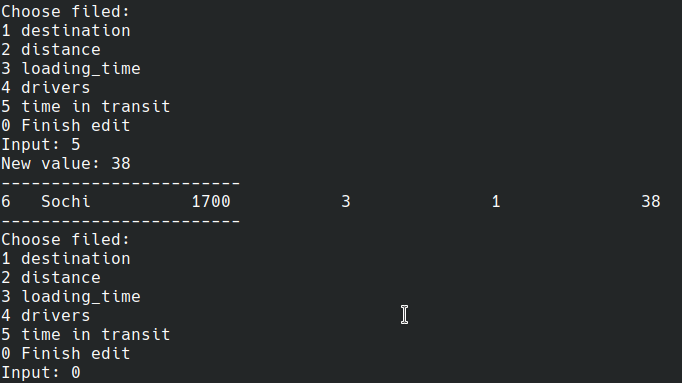
\includegraphics[width=0.8\linewidth]{photo/tests/admin/route_db_edit_3}
	\caption{Тест -- Редактирование записи из базы маршрутов (3)}
	\label{route_db_edit_3}
\end{figure}

\begin{figure}[H]
	\centering
	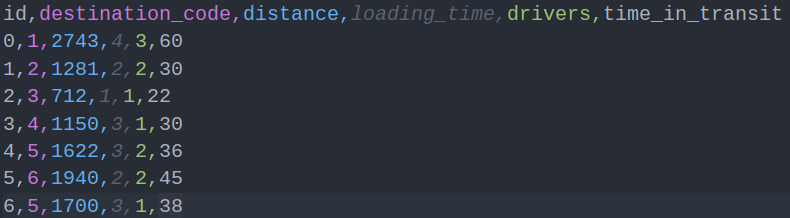
\includegraphics[width=0.7\linewidth]{photo/tests/admin/route_db_state_edit}
	\caption{Тест -- Файл базы данных маршрутов после изменений}
	\label{route_db_state_edit}
\end{figure}

Запустим консоль и введём пароль. 
Выберем базу маршрутов и удалим запись

Ожидается, что программа удалит элемент из файла базы данных.
Исходный файл с базой до изменений на рис. \ref{route_db_state_edit2}.
Результат выполнения на рис. \ref{route_db_delete}.
Исходный файл с базой после изменений на рис. \ref{route_db_state_init3}.

\begin{figure}[H]
	\centering
	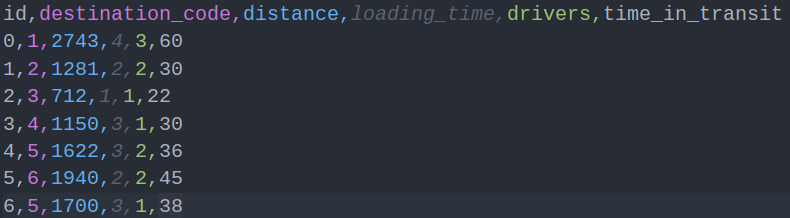
\includegraphics[width=0.7\linewidth]{photo/tests/admin/route_db_state_edit}
	\caption{Тест -- Файл базы данных маршрутов до изменений}
	\label{route_db_state_edit2}
\end{figure}

\begin{figure}[H]
	\centering
	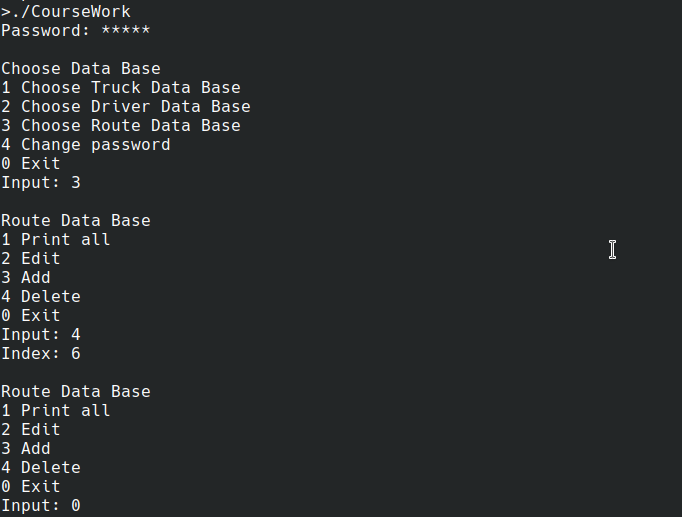
\includegraphics[width=0.8\linewidth]{photo/tests/admin/route_db_delete}
	\caption{Тест -- Удаление записи из базы маршрутов}
	\label{route_db_delete}
\end{figure}

\begin{figure}[H]
	\centering
	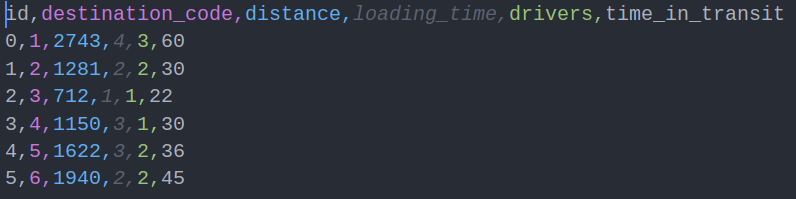
\includegraphics[width=0.7\linewidth]{photo/tests/admin/route_db_state_init}
	\caption{Тест -- Файл базы данных маршрутов после изменений}
	\label{route_db_state_init3}
\end{figure}

Запустим консоль и введём пароль. 
Выберем смену пароля и изменим пароль на новый.
Попытаемся войти в консоль со старым и новым паролем.

Ожидается, что программа обновит пароль и 
будет запускаться только с новым паролем.
Результат выполнения на рис. \ref{change_pass}.

\begin{figure}[H]
	\centering
	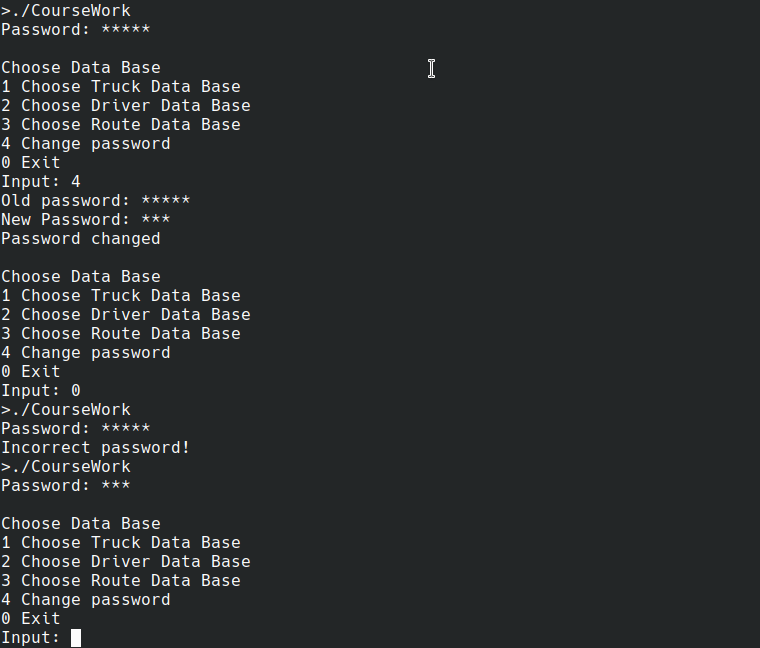
\includegraphics[width=0.7\linewidth]{photo/tests/admin/change_pass}
	\caption{Тест -- Смена пароля}
	\label{change_pass}
\end{figure}

\subsection{Тесты пользовательского интерфейса}

Тесты проводились на базах данных, указанных на рис. \ref{truck_db_}, \ref{driver_db_}, \ref{route_db_} (грузовики, водители и маршруты соответственно).

\begin{figure}[H]
	\centering
	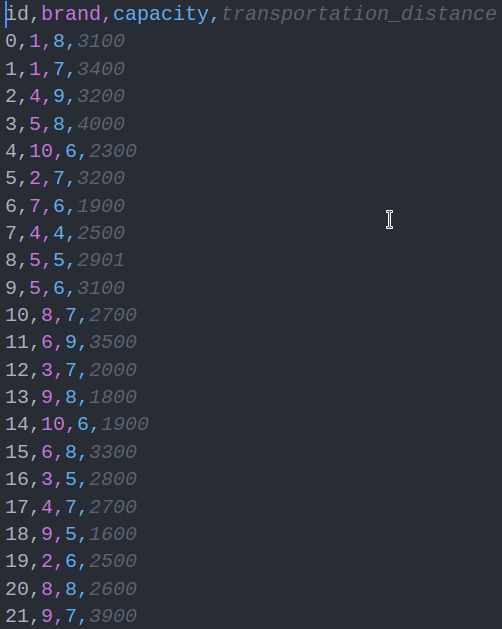
\includegraphics[width=0.7\linewidth]{photo/tests/user/truck_db}
	\caption{База данных грузовиков}
	\label{truck_db_}
\end{figure}

\begin{figure}[H]
	\centering
	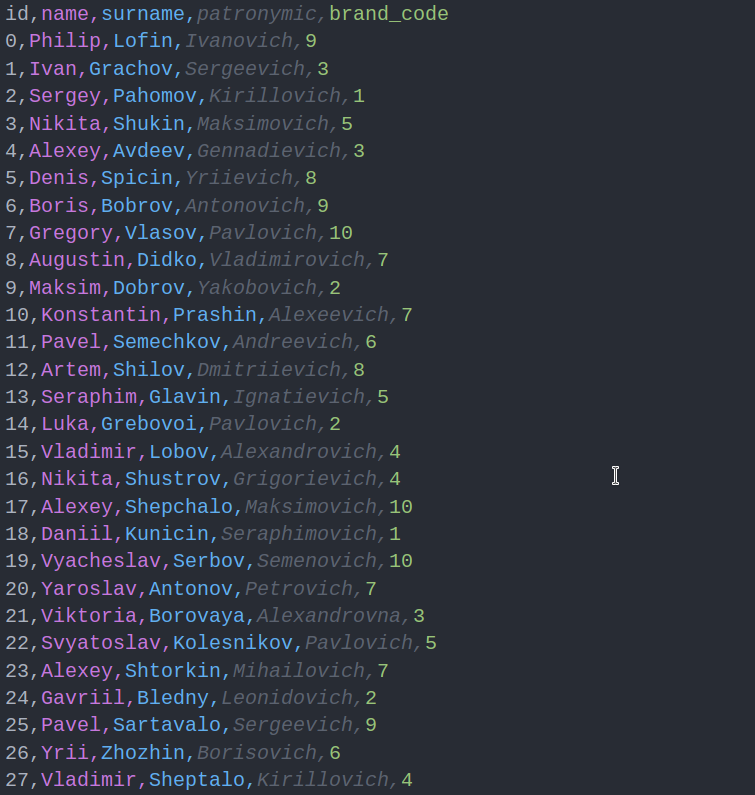
\includegraphics[width=0.7\linewidth]{photo/tests/user/driver_db}
	\caption{База данных водителей}
	\label{driver_db_}
\end{figure}

\begin{figure}[H]
	\centering
	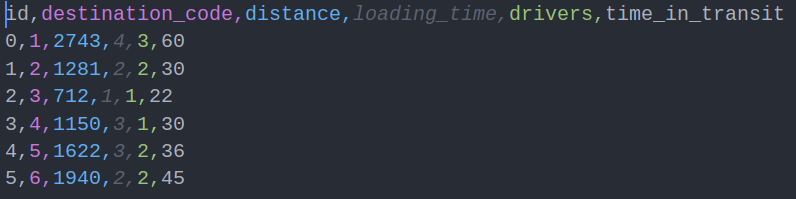
\includegraphics[width=0.7\linewidth]{photo/tests/user/route_db}
	\caption{База данных маршрутов}
	\label{route_db_}
\end{figure}

Отправим запрос в программу (рис. \ref{request_1}).

\begin{figure}[H]
	\centering
	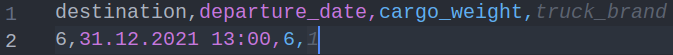
\includegraphics[width=0.7\linewidth]{photo/tests/user/request_1}
	\caption{Запрос для теста №1}
	\label{request_1}
\end{figure}

Ожидается, что программа успешно отработает --- выберет грузовик с идентификатором 0 
и водителей с идентификаторами 2 и 18, занесёт запись в расписание.

База расписания до отправки запроса на рис. \ref{schedule_db_init}.
Результат выполнения на рис. \ref{test_1}.
База расписания после обработки запроса на рис. \ref{schedule_db_test_1}.

\begin{figure}[H]
	\centering
	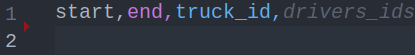
\includegraphics[width=0.7\linewidth]{photo/tests/user/schedule_db_init}
	\caption{База расписания до отправки запроса}
	\label{schedule_db_init}
\end{figure}

\begin{figure}[H]
	\centering
	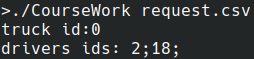
\includegraphics[width=0.7\linewidth]{photo/tests/user/test_1}
	\caption{Тест 1}
	\label{test_1}
\end{figure}

\begin{figure}[H]
	\centering
	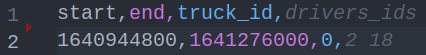
\includegraphics[width=0.7\linewidth]{photo/tests/user/schedule_db_test_1}
	\caption{База расписания после обработки запроса}
	\label{schedule_db_test_1}
\end{figure}

Повторно отправим тот же самый запрос в программу (рис. \ref{request_1_again}).

\begin{figure}[H]
	\centering
	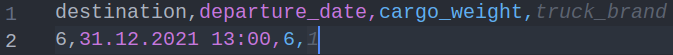
\includegraphics[width=0.7\linewidth]{photo/tests/user/request_1}
	\caption{Запрос для теста №2}
	\label{request_1_again}
\end{figure}

Ожидается, что программа выдаст ошибку --- 
не найдётся свободных водителей на заданную дату.

База расписания до отправки запроса на рис. \ref{schedule_db_21}.
Результат выполнения на рис. \ref{test_2}.
База расписания после обработки запроса на рис. \ref{schedule_db_22}.

\begin{figure}[H]
	\centering
	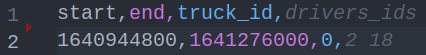
\includegraphics[width=0.7\linewidth]{photo/tests/user/schedule_db_test_1}
	\caption{База расписания до отправки запроса}
	\label{schedule_db_21}
\end{figure}

\begin{figure}[H]
	\centering
	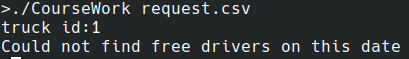
\includegraphics[width=0.7\linewidth]{photo/tests/user/test_2}
	\caption{Тест 2}
	\label{test_2}
\end{figure}

\begin{figure}[H]
	\centering
	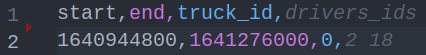
\includegraphics[width=0.7\linewidth]{photo/tests/user/schedule_db_test_1}
	\caption{База расписания после обработки запроса}
	\label{schedule_db_22}
\end{figure}

Отправим запрос в программу (рис. \ref{request_2}).

\begin{figure}[H]
	\centering
	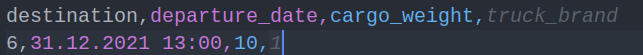
\includegraphics[width=0.7\linewidth]{photo/tests/user/request_2}
	\caption{Запрос для теста №3}
	\label{request_2}
\end{figure}

Ожидается, что программа выдаст ошибку --- 
не найдётся подходящих грузовиков на заданную дату.

База расписания до отправки запроса на рис. \ref{schedule_db_31}.
Результат выполнения на рис. \ref{test_3}.
База расписания после обработки запроса на рис. \ref{schedule_db_32}.

\begin{figure}[H]
	\centering
	\includegraphics[width=0.7\linewidth]{photo/tests/user/schedule_db_test_1}
	\caption{База расписания до отправки запроса}
	\label{schedule_db_31}
\end{figure}

\begin{figure}[H]
	\centering
	\includegraphics[width=0.7\linewidth]{photo/tests/user/test_3}
	\caption{Тест 3}
	\label{test_3}
\end{figure}

\begin{figure}[H]
	\centering
	\includegraphics[width=0.7\linewidth]{photo/tests/user/schedule_db_test_1}
	\caption{База расписания после обработки запроса}
	\label{schedule_db_32}
\end{figure}

Отправим запрос в программу (рис. \ref{request_3}).

\begin{figure}[H]
	\centering
	\includegraphics[width=0.7\linewidth]{photo/tests/user/request_3}
	\caption{Запрос для теста №4}
	\label{request_3}
\end{figure}

Ожидается, что программа выдаст ошибку --- 
запрошенная дата уже прошла.

База расписания до отправки запроса на рис. \ref{schedule_db_41}.
Результат выполнения на рис. \ref{test_4}.
База расписания после обработки запроса на рис. \ref{schedule_db_42}.

\begin{figure}[H]
	\centering
	\includegraphics[width=0.7\linewidth]{photo/tests/user/schedule_db_test_1}
	\caption{База расписания до отправки запроса}
	\label{schedule_db_41}
\end{figure}

\begin{figure}[H]
	\centering
	\includegraphics[width=0.7\linewidth]{photo/tests/user/test_4}
	\caption{Тест 4}
	\label{test_4}
\end{figure}

\begin{figure}[H]
	\centering
	\includegraphics[width=0.7\linewidth]{photo/tests/user/schedule_db_test_1}
	\caption{База расписания после обработки запроса}
	\label{schedule_db_42}
\end{figure}